\subsection{Excercise CarRentalStructs}
\label{sec:car_rental_structs}
% TODO Einleitung zu jeder Aufgabe schreiben

\subsubsection*{Add the Attributes to Structs}
After adding the attributes from the entity diagram to the 
\texttt{.../golang/CarRental/CarRentalStructs/CarRentalStructs.go} path and saving
the IDE automatically formats the code and indents it correctly.

\subsubsection*{Initialize and Print Structs}
The result of the initialization and printing of the structs is shown in figure \ref{fig:car_rental_structs}.
\begin{figure}[H]
    \centering
    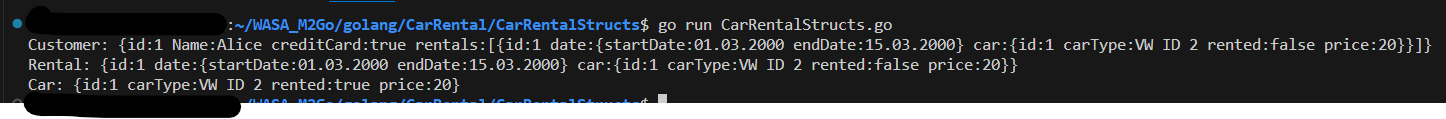
\includegraphics[width=\textwidth]{figures/goLang/carRental/carRental_structs.png}
    \caption{Output of the structs}
    \label{fig:car_rental_structs}
\end{figure}

\subsubsection*{Create an Array of Rentals}
The function works as follows:
\begin{enumerate}
    \item The array \texttt{cartypes} holds the string of 5 different cartypes
    \item The function \texttt{createRentals(id, date, car)} returns 5 rentals that are appended to the array
    \item Via \texttt{fmt.Println(rentals)} the array is printed into the console
\end{enumerate}

The result is shown in figure \ref{fig:car_rental_array_five_rentals}.

The initialization process of an empty array containing 5 cars in go looks as follows: \texttt{var cars \[5\]Car}
Alternatively the array can be created already initialized with \texttt{var cartypes = \[5\]string\{"Type1", ..., "Type5"\}}
This notation creates an array of 5 strings representing cartypes.

A for loop in go ranges from an integer value, usually called "i", to an upper border.
The value will usually be incremented by one until the upper border is reached. 
The code within the loop will be executed until i reaches the upper border.
A correct implementation for five iterations is shown in listing \ref{lst:for_loop_init}.

\begin{lstlisting}[
    language=Golang,
    caption={Initialization of a For-Loop iterating five Times},
    label={lst:for_loop_init},
    numbers=left,
    numberstyle=\tiny
]
    for i := 0; i < 5; i++ {
        // run some code
    }
\end{lstlisting}

\begin{figure}[H]
    \centering
    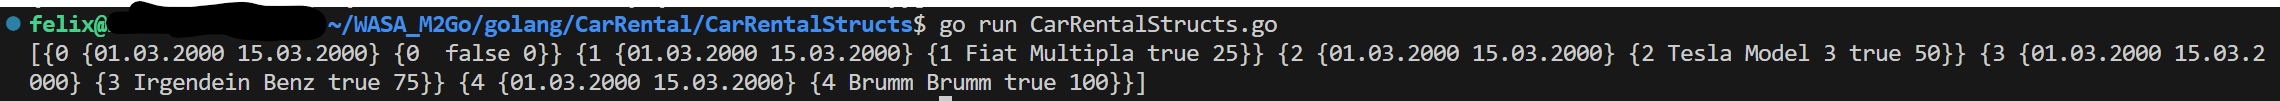
\includegraphics[width=\textwidth]{figures/goLang/carRental/carRental_arrayFiveRentals.png}
    \caption{Output of the Array of Rentals}
    \label{fig:car_rental_array_five_rentals}
\end{figure}

\subsection{Excercise CarRentalTests}
\label{sec:car_rental_tests}
\subsubsection*{Analyze OCL Constraints}
In the given task five invariants are described.
These invariants are implemented in \texttt{./CarRentalTests/CarRentalTests.go} and executed in \texttt{./CarRentalStructs/CarRentalStructs.go}.
\begin{enumerate}
    \item \texttt{self.Date.Year >= 2000}: CarRentalTests.go line 20-22
    \item \texttt{self.Date.Month < 13}: CarRentalTests.go line 24-26
    \item \texttt{self.Date.Moth >= 1}: CarRentalTests.go line 24-26
    \item \texttt{self.ValidateNumberOfDaysInMonth() == True}: CarRentalTests.go line 32
\end{enumerate}

\subsubsection*{Run Test}
After running the test function an error occurs. 
The test, therefore, does not pass.
The error is shown in figure \ref{fig:car_rental_test_error}.

This error is caused due to a false implementation in line 20 of \texttt{./CarRentalTests/CarRentalTests.go}
In the first test, it checks if the year is $>2000$, yet for correct execution it needs to be $>=2000$.

\begin{figure}[H]
    \centering
    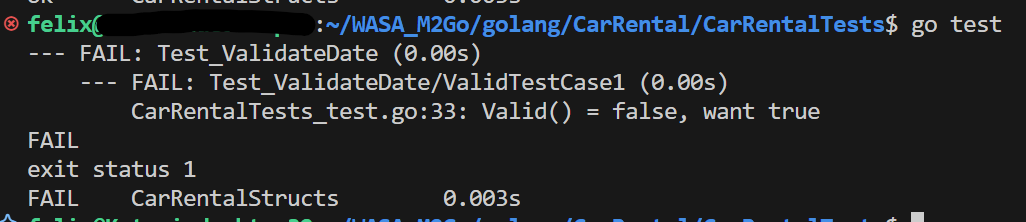
\includegraphics[width=0.8\textwidth]{figures/goLang/carRental/carRental_dateTestError.png}
    \caption{Error of the Test}
    \label{fig:car_rental_test_error}
\end{figure}

\subsubsection*{Correct Code}
As mentioned in the subsection above, line 20 is not implemented correctly.
By changing line 20 from \texttt{if !(d.Year \> 2000)} to \texttt{if !(d.Year \>\= 2000)} the code will execute correctly and the test passes.
The working tree of the changes is shown in figure \ref{fig:car_rental_test_working_tree}.

\begin{figure}[H]
    \centering
    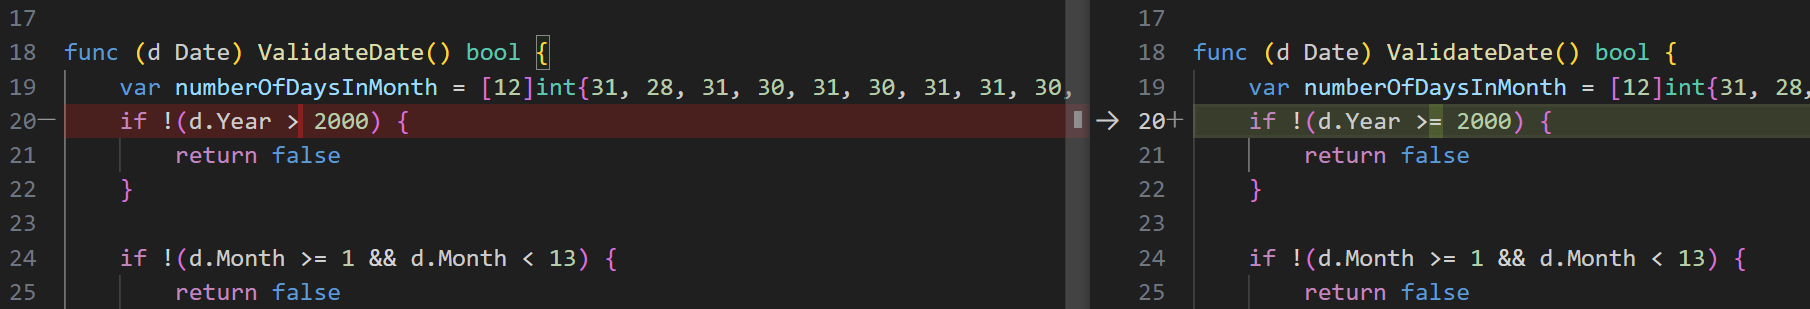
\includegraphics[width=\textwidth]{figures/goLang/carRental/carRental_dateTestWorkingTree.png}
    \caption{Working Tree of the Changes}
    \label{fig:car_rental_test_working_tree}
\end{figure}

\subsubsection*{Negative Test Case}
Implementing an invalid test-case the following code is added to the test function:
\begin{lstlisting}[
    language=Golang,
    numbers=left,
    numberstyle=\tiny,
    caption={Invalid Test Case},
    label={lst:invalid_test_case}
    ]
	    name:   "InvalidTestCase1",
        fields: fields{Day: 12, Month: 13, Year: 2000},
	    want:   false,  
\end{lstlisting}

As shown in listing \ref{lst:invalid_test_case} the month is set to 13, which is invalid.
Therefore the test should return false.
The test, however, runs succesfully due to the want value set to false.
